\section{Curve Sketching}
\label{sec:sketching}

This section examines some of the interplay between the shape of the graph of $f(x)$ and the behavior of $f'(x)$. If we have a graph of $f(x)$, we will see what we can conclude about the values of $f'(x)$. If we know values of $f'(x)$, we will see what we can conclude about the graph of $f(x)$. We will also utilize the information from $f''(x)$ that we learned in the last section.

\subsection{First Derivative Information}
\begin{definition}
Suppose that a function $f(x)$ is defined on the open interval $(a, b)$.
    \begin{itemize}[label={}]
    \item The function $f(x)$ is {\bf increasing}\index{Increasing} on $(a,b)$ if $a<x_1<x_2<b$ implies $f(x_1)<f(x_2)$.
    \item The function $f(x)$ is {\bf decreasing}\index{Decreasing} on $(a,b)$ if $a<x_1<x_2<b$ implies $f(x_1)>f(x_2)$.
    \end{itemize}
\end{definition}
Graphically, $f(x)$ is increasing (decreasing) if, as we move from left to right along the graph of $f(x)$, the height of the graph increases (decreases).

These same ideas make sense if we consider $h(t)$ to be the height (in feet) of a rocket $t$ seconds after liftoff. We naturally say that the rocket is rising or that its height is increasing if the height $h(t)$ increases over a period of time, as $t$ increases.

\begin{example}
List the intervals on which the function shown is increasing or decreasing.

\begin{figure}[!ht]
  \centering
    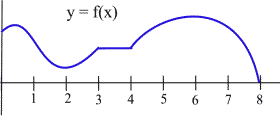
\includegraphics[width=0.4\textwidth]{img/chap3/image072.png}
    %\caption{Visualizing the Second Derivative Test}
    %\label{fig:3-4-2derivtest}
\end{figure}
\begin{solution} $f(x)$ is increasing on the intervals $[0,0.5)$, $(2,3)$ and $(4,6)$. Notice that we don't include critical values\index{Critical value} in the intervals. A function is neither increasing nor decreasing at a critical point\index{Critical point}\index{Point!critical}.

$f(x)$ is decreasing on $(0.5,2)$ and $(6,8)$.

On the interval $[3,4]$, $f(x)$ is neither increasing nor decreasing -- it is constant.
\end{solution}\end{example}

\begin{theorem}[First Derivative Information about Shape (Part 1)]
\label{thm:3-5-shape1}
Let $f(x)$ be a function which is differentiable on an interval $(a,b)$.
    \begin{itemize}
    \item If $f(x)$ is increasing on $(a,b)$, then $f'(x)\ge 0$ for all $x$ in $(a,b)$.
    \item If $f(x)$ is decreasing on $(a,b)$, then $f'(x)\le 0$ for all $x$ in $(a,b)$.
    \item If $f(x)$ is constant on $(a,b)$, then $f'(x)=0$ for all $x$ in $(a,b)$.
    \end{itemize}
\end{theorem}
\begin{example}
The graph in Figure \ref{fig:3-5-helicopter} shows the elevation of a helicopter during a period of time. Sketch the graph of the upward velocity of the helicopter, $\dfrac{dh}{dt}$.

\begin{figure}[!ht]
  \centering
    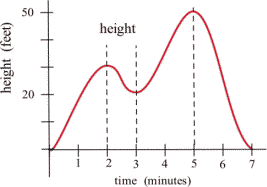
\includegraphics[width=0.4\textwidth]{img/chap3/image073.png}
    \caption{Elevation of a Helicopter}
    \label{fig:3-5-helicopter}
\end{figure}
\begin{solution} Notice that $h(t)$ has a local maximum when $t=2$ and $t=5$, so $v(2)=0$ and $v(5)=0$, where $v(t) = h'(t)$ is the upward velocity of the helicopter. Similarly, $h(t)$ has a local minimum when $t=3$, so $v(3)=0$.

When $h(x)$ is increasing, $v(t)>0$. When $h(t)$ is decreasing, $v(t)<0$.

Using this information, we can sketch a graph of $v(t)=\dfrac{dh}{dt}$.

\begin{figure}[!ht]
  \centering
    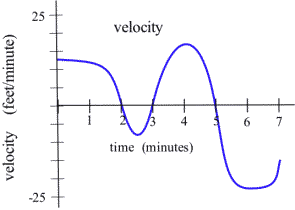
\includegraphics[width=0.4\textwidth]{img/chap3/image074.png}
    \caption{Vertical Velocity of the Helicopter}
    \label{fig:3-5-helicopterv}
\end{figure}
\end{solution}\end{example}

The next theorem is almost the converse of the First Shape Theorem (Theorem \ref{thm:3-5-shape1}) and explains the relationship between the values of the derivative and the graph of a function from a different perspective. It says that if we know something about the values of $f'(x)$, then we can draw some conclusions about the shape of the graph of $f(x)$.

\begin{theorem}[First Derivative Information about Shape (Part 2)]
Let $f(x)$ be a function which is differentiable on an interval $I$.
    \begin{itemize}
    \item If $f'(x)>0$ for all $x$ in the interval $I$, then $f(x)$ is {\bf increasing}\index{Increasing} on $I$.
    \item If $f'(x)<0$ for all $x$ in the interval $I$, then $f(x)$ is {\bf decreasing}\index{Decreasing} on $I$.
    \item If $f'(x)=0$ for all $x$ in the interval $I$, then $f(x)$ is {\bf constant}\index{Constant} on $I$.
    \end{itemize}
\end{theorem}
\begin{example}
Use information about the values of $f'(x)$ to help graph $f(x)=x^3-6x^2+9x+1$.

\begin{solution} $f'(x)=3x^2-12x+9=3(x-1)(x-3)$, so $f'(x)=0$ only when $x=1$ or $x=3$. $f'(x)$ is a polynomial so it is always defined.

The only critical numbers for $f(x)$ are $x=1$ and $x=3$, and they divide the real number line into three intervals: $(-\infty,1)$, $(1,3)$, and $(3,\infty)$. On each of these intervals, the function is either always increasing or always decreasing.
    \begin{itemize}[label={}]
    \item If $x<1$, then $f'(x)= 3(-)(-)>0$, so $f(x)$ is increasing.
    \item If $1<x<3$, then $f'(x)= 3(+)(-) <0$, so $f(x)$ is decreasing.
    \item If $x>3$, then $f'(x)= 3(+)(+) >0$, so $f(x)$ is increasing.
    \end{itemize}
Even though we don't know the value of $f(x)$ anywhere yet, we do know a lot about the shape of the graph of $f(x)$: as we move from left to right along the $x$-axis, the graph of $f(x)$ increases until $x=1$, then the graph decreases until $x=3$, and then the graph increases again. The graph of $f(x)$ makes ``turns'' when $x=1$ and $x=3$; it has a local maximum at $x=1$, and a local minimum at $x=3$. Figure \ref{fig:3-5-signs} sketches this information.

\begin{figure}[!ht]
  \centering
    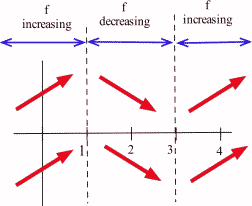
\includegraphics[width=0.4\textwidth]{img/chap3/image075.png}
    \caption{Sketching where $f(x)$ increases and decreases.}
    \label{fig:3-5-signs}
\end{figure}
To plot the graph of $f(x)$, we still need to evaluate $f(x)$ at a few values of $x$, but only at a very few values. $f(1)=5$, and $(1,5)$ is a local maximum of $f(x)$. $f(3)=1$, and $(3,1)$ is a local minimum of $f(x)$. The resulting graph of $f(x)$ is shown in Figure \ref{fig:3-5-fx}.

\begin{figure}[!ht]
  \centering
    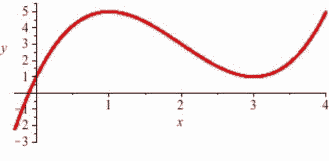
\includegraphics[width=0.4\textwidth]{img/chap3/image076.png}
    \caption{Sketch of $y=f(x)$}
    \label{fig:3-5-fx}
\end{figure}
\end{solution}\end{example}

\subsection{Second Derivative Information}
Until now, we've only used first derivative information, but we could also use information from the second derivative to provide more information about the shape of the function.

\begin{theorem}[Second Derivative Information about Shape]
Suppose $f(x)$ is continuous and both $f'(x)$ and $f''(x)$ exist on the interval $(a, b)$.
    \begin{itemize} 
    \item If $f(x)$ is concave up\index{Concave up} on $(a,b)$, then $f''(x)\ge 0$ for all $x$ in $(a,b)$.
    \item If $f(x)$ is concave down\index{Concave down} on $(a,b)$, then $f''(x)\le 0$ for all $x$ in $(a,b)$.
    \end{itemize}
The converse of both of these are also true.
    \begin{itemize}
    \item If $f''(x)\ge 0$ for all $x$ in $(a,b)$, then $f(x)$ is {\bf concave up}\index{Concave up} on $(a,b)$.
    \item If $f''(x)\le 0$ for all $x$ in $(a,b)$, then $f(x)$ is {\bf concave down}\index{COncave down} on $(a,b)$.
    \end{itemize}
\end{theorem}
\begin{example}
Use information about the values of $f''(x)$ to help determine the intervals on which the graph of the function $f(x)=x^3-6x^2+9x+1$ is concave up and concave down.

\begin{solution} For concavity, we need the second derivative: $f'(x)=3x^2-12x+9$, so $f''(x)=6x-12$.

To find possible inflection points, set the second derivative equal to zero. $6x-12=0$, so $x=2$. This divides the real number line into two intervals: $(-\infty, 2)$ and $(2, \infty)$.

For $x<2$, the second derivative is negative (for example, $f''(0)=6(0)-12=-12$), so $y=f(x)$ is concave down. For $x>2$, the second derivative is positive, so $y=f(x)$ is concave up.

We could have incorporated this concavity information when sketching the graph for the previous example, and indeed we can see the concavity reflected in the graph shown.
\end{solution}\end{example}

\begin{example}
Use information about the values of $f'(x)$ and $f''(x)$ to help graph $f(x)=x^{2/3}$.

\begin{solution} $f'(x)=\dfrac{2}{3}x^{-1/3}$. This is undefined at $x=0$.

$f''(x)=\dfrac{-2}{9}x^{-4/3}$. This is also undefined at $x=0$.

This creates two intervals: $x<0$, and $x>0$.

On the interval $x<0$, we could test out a value like $x=-1$:
$$f'(-1)=\dfrac{2}{3}(-1)^{-1/3}=-\dfrac{2}{3}<0$$
and
$$f''(-1)=-\dfrac{2}{9}(-1)^{-4/3}=-\dfrac{2}{9}<0 \enspace .$$
$f'(-1)$ is negative and $f''(-1)$ is negative, so we can conclude that $f(x)$ is decreasing and concave down on the interval $(-\infty, 0)$.

On the interval $x>0$, we could test out a value like $x=1$:
$$f'(1)=\dfrac{2}{3}(1)^{-1/3}=\dfrac{2}{3} > 0$$
and
$$f''(1)=-\dfrac{2}{9}(1)^{-4/3}=-\dfrac{2}{9} < 0 \enspace .$$
$f'(1)$ is positive and $f''(1)$ is negative, so we can conclude that $f(x)$ is increasing and concave down on the interval $(0, \infty)$.

We can also calculate that $f(0)=0^{2/3} = 0$, giving us a base point for the graph. Using this information, we can conclude the graph must look like this.

\begin{figure}[!ht]
  \centering
    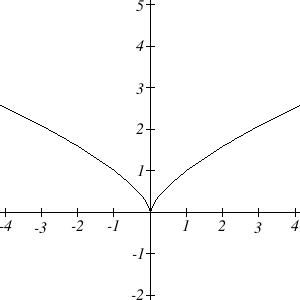
\includegraphics[width=0.4\textwidth]{img/chap3/image077.png}
    \caption{Sketch of $y=x^{2/3}$}
    \label{fig:3-5-ex5}
\end{figure}
\end{solution}\end{example}

\subsection{Sketching without an Equation}
Of course, graphing calculators and computers are great at graphing functions. Calculus provides a way to illuminate what may be hidden or out of view when we graph using technology. More importantly, calculus gives us a way to look at the derivatives of functions for which there is no equation given. We already saw the idea of this back in Section \ref{sec:derivative}, where we sketched the derivative of two graphs by estimating slopes on the curves.

We can summarize all the derivative information about shape in a table.
\begin{theorem}
\begin{table}[!ht]
    \centering
    \begin{tabular}{lllll}
    \toprule    
    $f(x)$      & Increasing	& Decreasing	& Concave Up	& Concave Down	\\
    \midrule
    $f'(x)$     & $+$	        & $-$	        & Increasing	& Decreasing	\\
    \midrule
    $f''(x)$	&               & 	            & $+$	        & $-$\\
    \bottomrule
    \end{tabular}
    \caption{Summary of Derivative Information about the Graph}
    \label{tab:3-5-analysis}
\end{table}
\begin{itemize}[label={}]
    \item When $f'(x)=0$, the graph of $f(x)$ may have a local maximum or minimum.
    \item When $f''(x)=0$, the graph of $f(x)$ may have an inflection point\index{Inflection point}\index{Point!inflection}.
\end{itemize}
\end{theorem}

\begin{example}
A company's bank balance, $B$, in millions of dollars, $t$ weeks after releasing a new product is shown in Figure \ref{fig:3-5-balance}. Sketch a graph of the marginal balance -- the rate at which the bank balance was changing over time.

\begin{figure}[!ht]
  \centering
    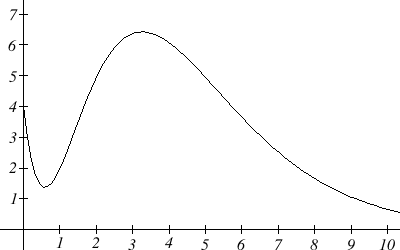
\includegraphics[width=0.4\textwidth]{img/chap3/image078.png}
    \caption{Company Balance after $t$ Years}
    \label{fig:3-5-balance}
\end{figure}

\begin{solution} Notice that since the tangent line of $y=B(t)$ will be horizontal at about $t=0.6$ and $t=3.2$; the derivative will be 0 at those points.

We can then identify intervals on which the original function is increasing or decreasing. This will tell us when the derivative function, $B'(t)$, is positive or negative.
\begin{table}[!ht]
    \centering
    \begin{tabular}{lll}
    \toprule 
    Interval	& $B(t)$        & $B'(t)$	\\
    \midrule 
    $0<t<0.6$   & Decreasing	& Negative	\\
    $0.6<t<3.2$ & Increasing	& Positive	\\
    $t>3.2$     & Decreasing	& Negative  \\
    \bottomrule
    \end{tabular}
\end{table}
There appear to be inflection points at about $t=1.5$ and $t=5.5$. At these points, the derivative will be changing from increasing to decreasing or vice versa, so the derivative will have a local maximum or minimum at those points.

Let's look at the intervals of concavity.
\begin{table}[!ht]
    \centering
    \begin{tabular}{lll}
    \toprule 
    Interval    & $y=B(t)$      & $B'(t)$ \\
    \midrule    
    $0<t<1.5$   & Concave Up    & Increasing \\
	$1.5<t<5.5$ & Concave Down	& Decreasing \\	
    $t>5.5$     & Concave Up	& Increasing \\
    \bottomrule
    \end{tabular}
\end{table}

If we wanted a more accurate sketch of the derivative function, we could also estimate the derivative at a few points by sketching a collection of tangent lines.
\begin{table}[!ht]
    \centering
    \begin{tabular}{lr}
    \toprule 
    $t$     & $B'(t)$\\
    $0$     & $-10$ \\	
    $1.5$	& $3$	\\
    $6$     & $-1$ \\
    \bottomrule
    \end{tabular}
\end{table}
\begin{figure}[!ht]
  \centering
    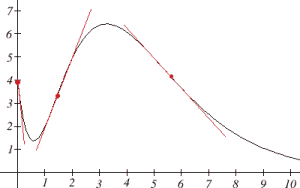
\includegraphics[width=0.4\textwidth]{img/chap3/image079.png}
    %\caption{Company Balance with tangent Lines}
    %\label{fig:3-5-balancetangents}
\end{figure}

Now we can sketch the derivative. We know a few values for the derivative function, and on each interval we know the shape we need. We can use this to create a rough idea of what the graph should look like.
\begin{figure}[!ht]
  \centering
    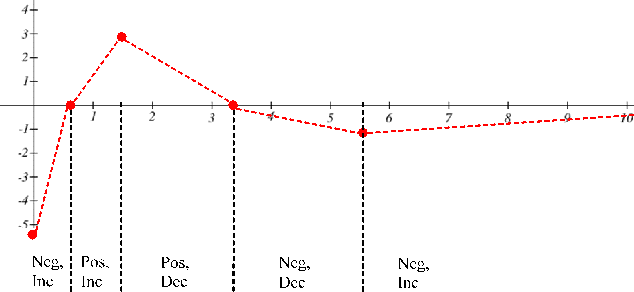
\includegraphics[width=0.4\textwidth]{img/chap3/image080.png}
    %\caption{Marginal Balance Sketch}
    %\label{fig:3-5-Bprimesketch}
\end{figure}

Smoothing this out gives us a good estimate for the graph of the derivative.
\begin{figure}[!ht]
  \centering
    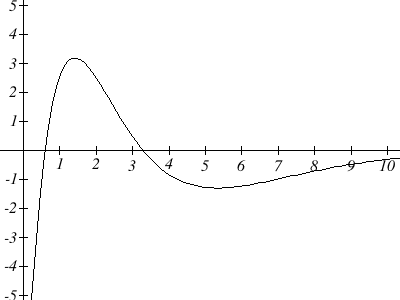
\includegraphics[width=0.4\textwidth]{img/chap3/image081.png}
    %\caption{Marginal Balance}
    %\label{fig:3-5-Bprime}
\end{figure}

\end{solution}\end{example}
